\subsection{Façade}
\label{facade}

\textbf{Scopo}: Strutturale \\
\textbf{Raggio d'azione}: Oggetti

\paragraph{Definizione} Il pattern Façade fornisce un'interfaccia unificata per un insieme di interfacce presenti in un sottosistema. Definisce un'interfaccia di livello più alto che rende il sistema più semplice da utilizzare.

\begin{figure}[H]
    \centering
    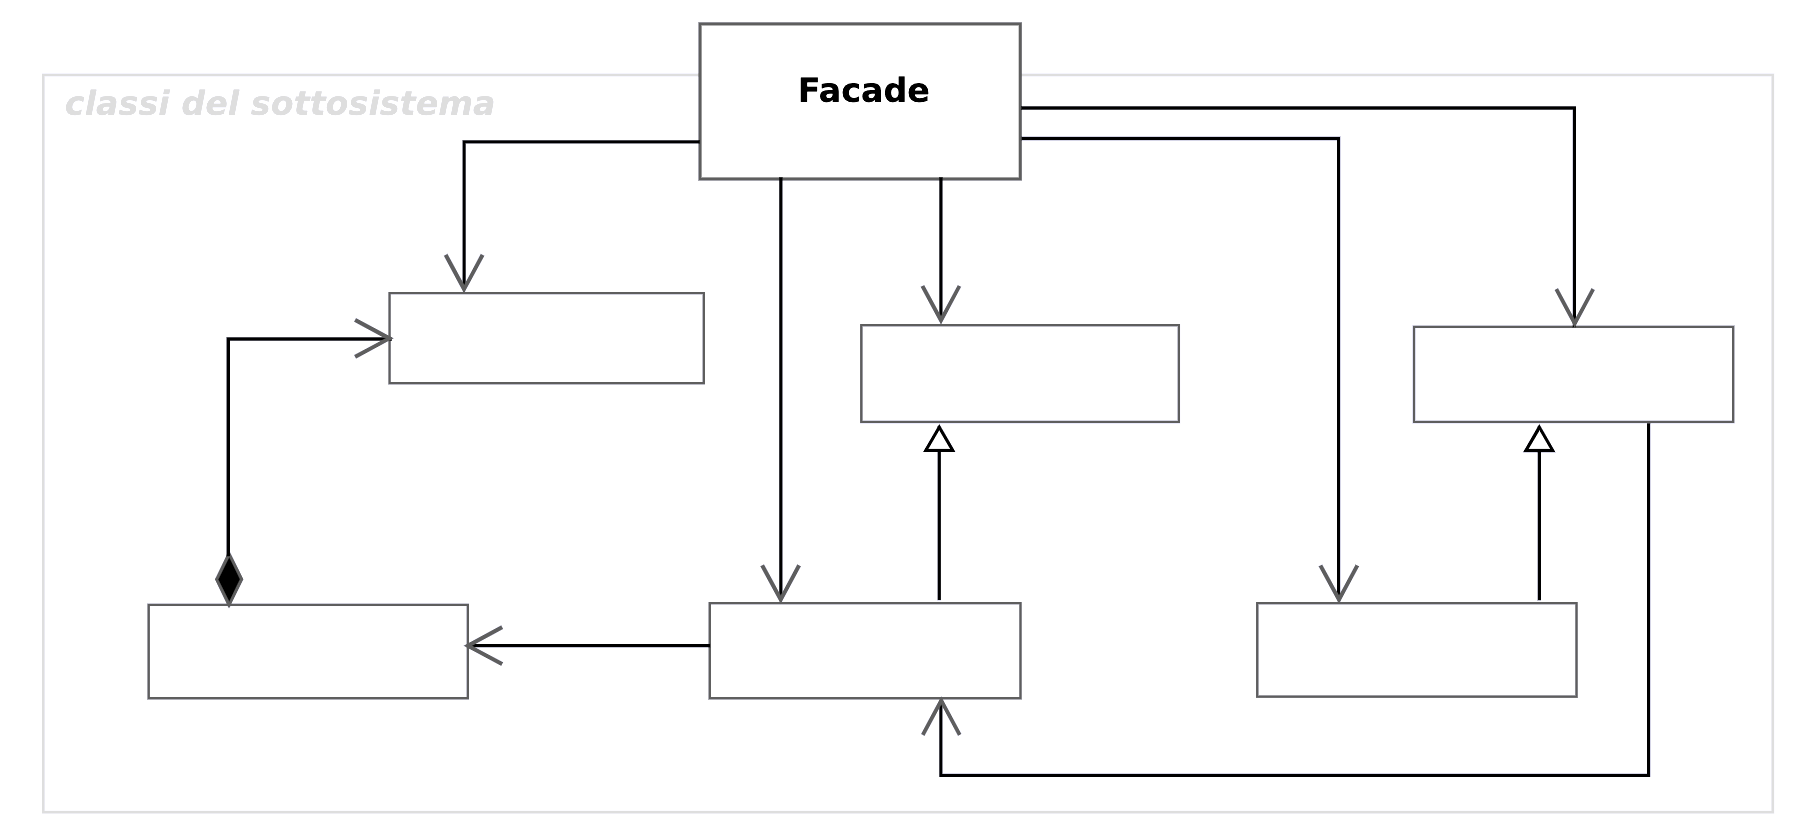
\includegraphics[width=1\linewidth]{assets/pattern/facade/facade-struttura.png}
    \caption{Class Diagram del pattern Façade}
\end{figure}

\paragraph{Struttura e Conseguenze} Il pattern Façade è composto da:
\begin{itemize}
    \item \textbf{Façade} (MessageCreator): conosce le classi nel sottosistema che sono responsabili di gestire una richiesta. 
    \item \textbf{Classi del sottosistema} (Message,MessageBody, Attachment, etc.): Implementano le funzionalità del sottosistema. Non hanno alcuna conoscenza dell’esistenza del Façade: non hanno alcun riferimento ad esso.
\end{itemize}

\begin{figure}[H]
    \centering
    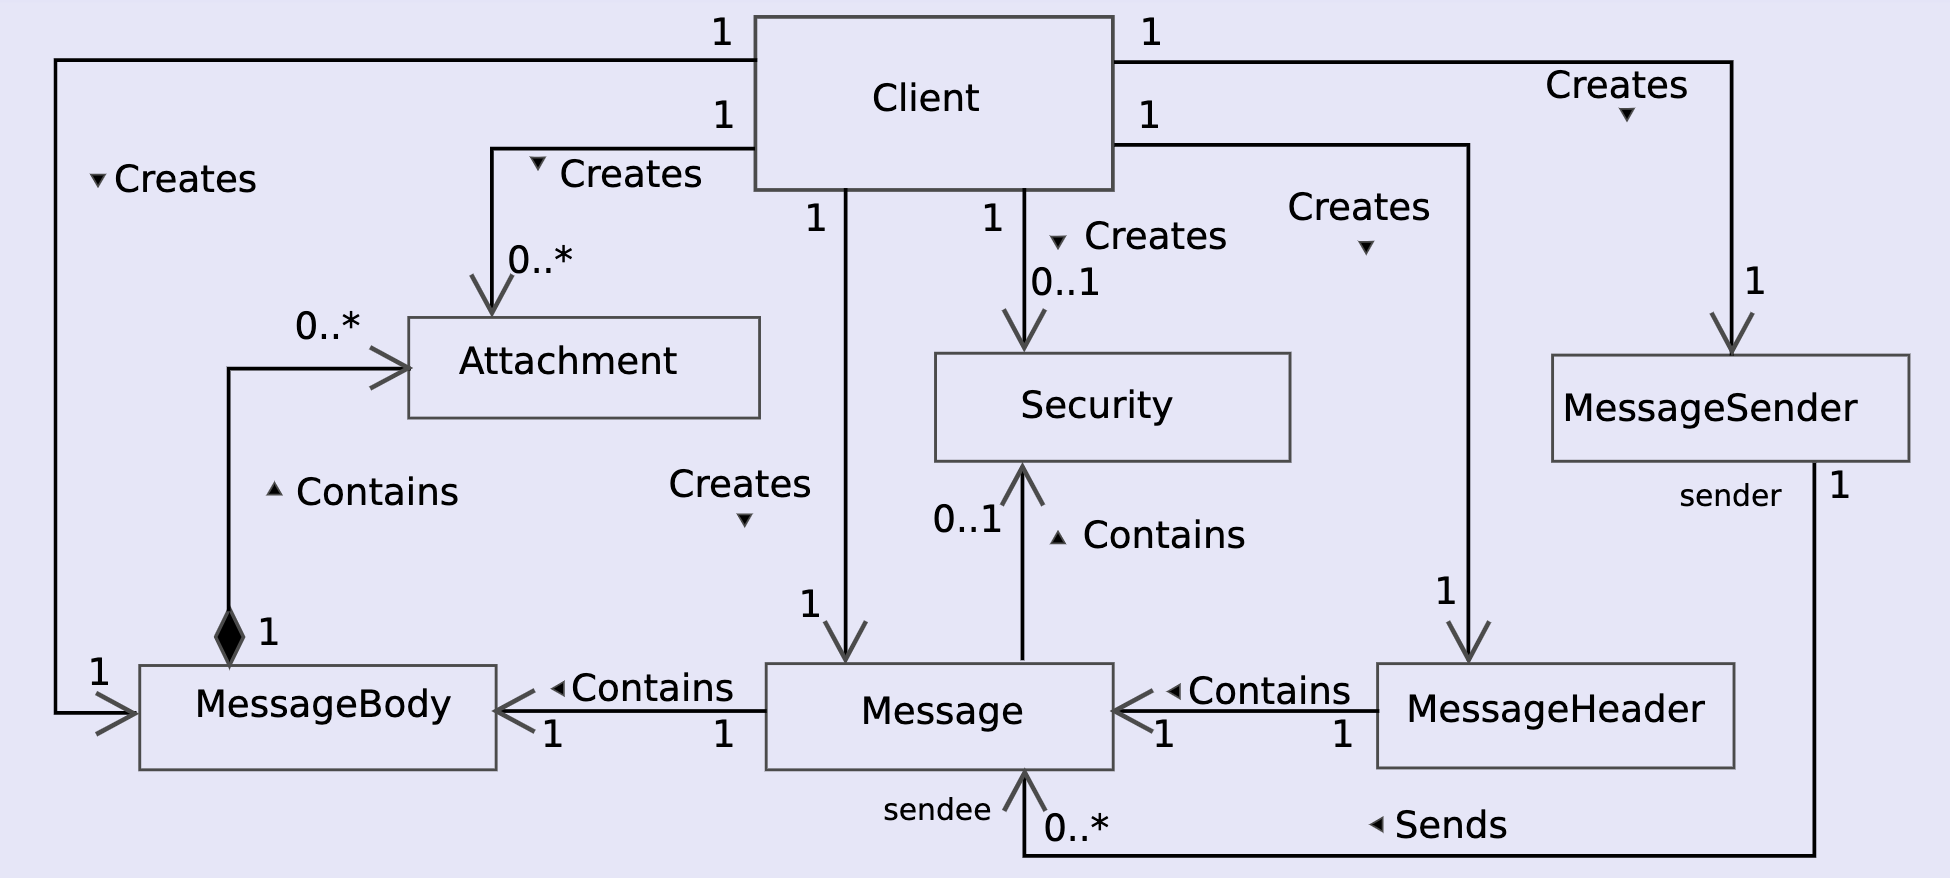
\includegraphics[width=1\linewidth]{assets/pattern/facade/facade-problema.png}
    \caption{Problema: creazione di un messaggio e-mail}
\end{figure}

\begin{figure}[H]
    \centering
    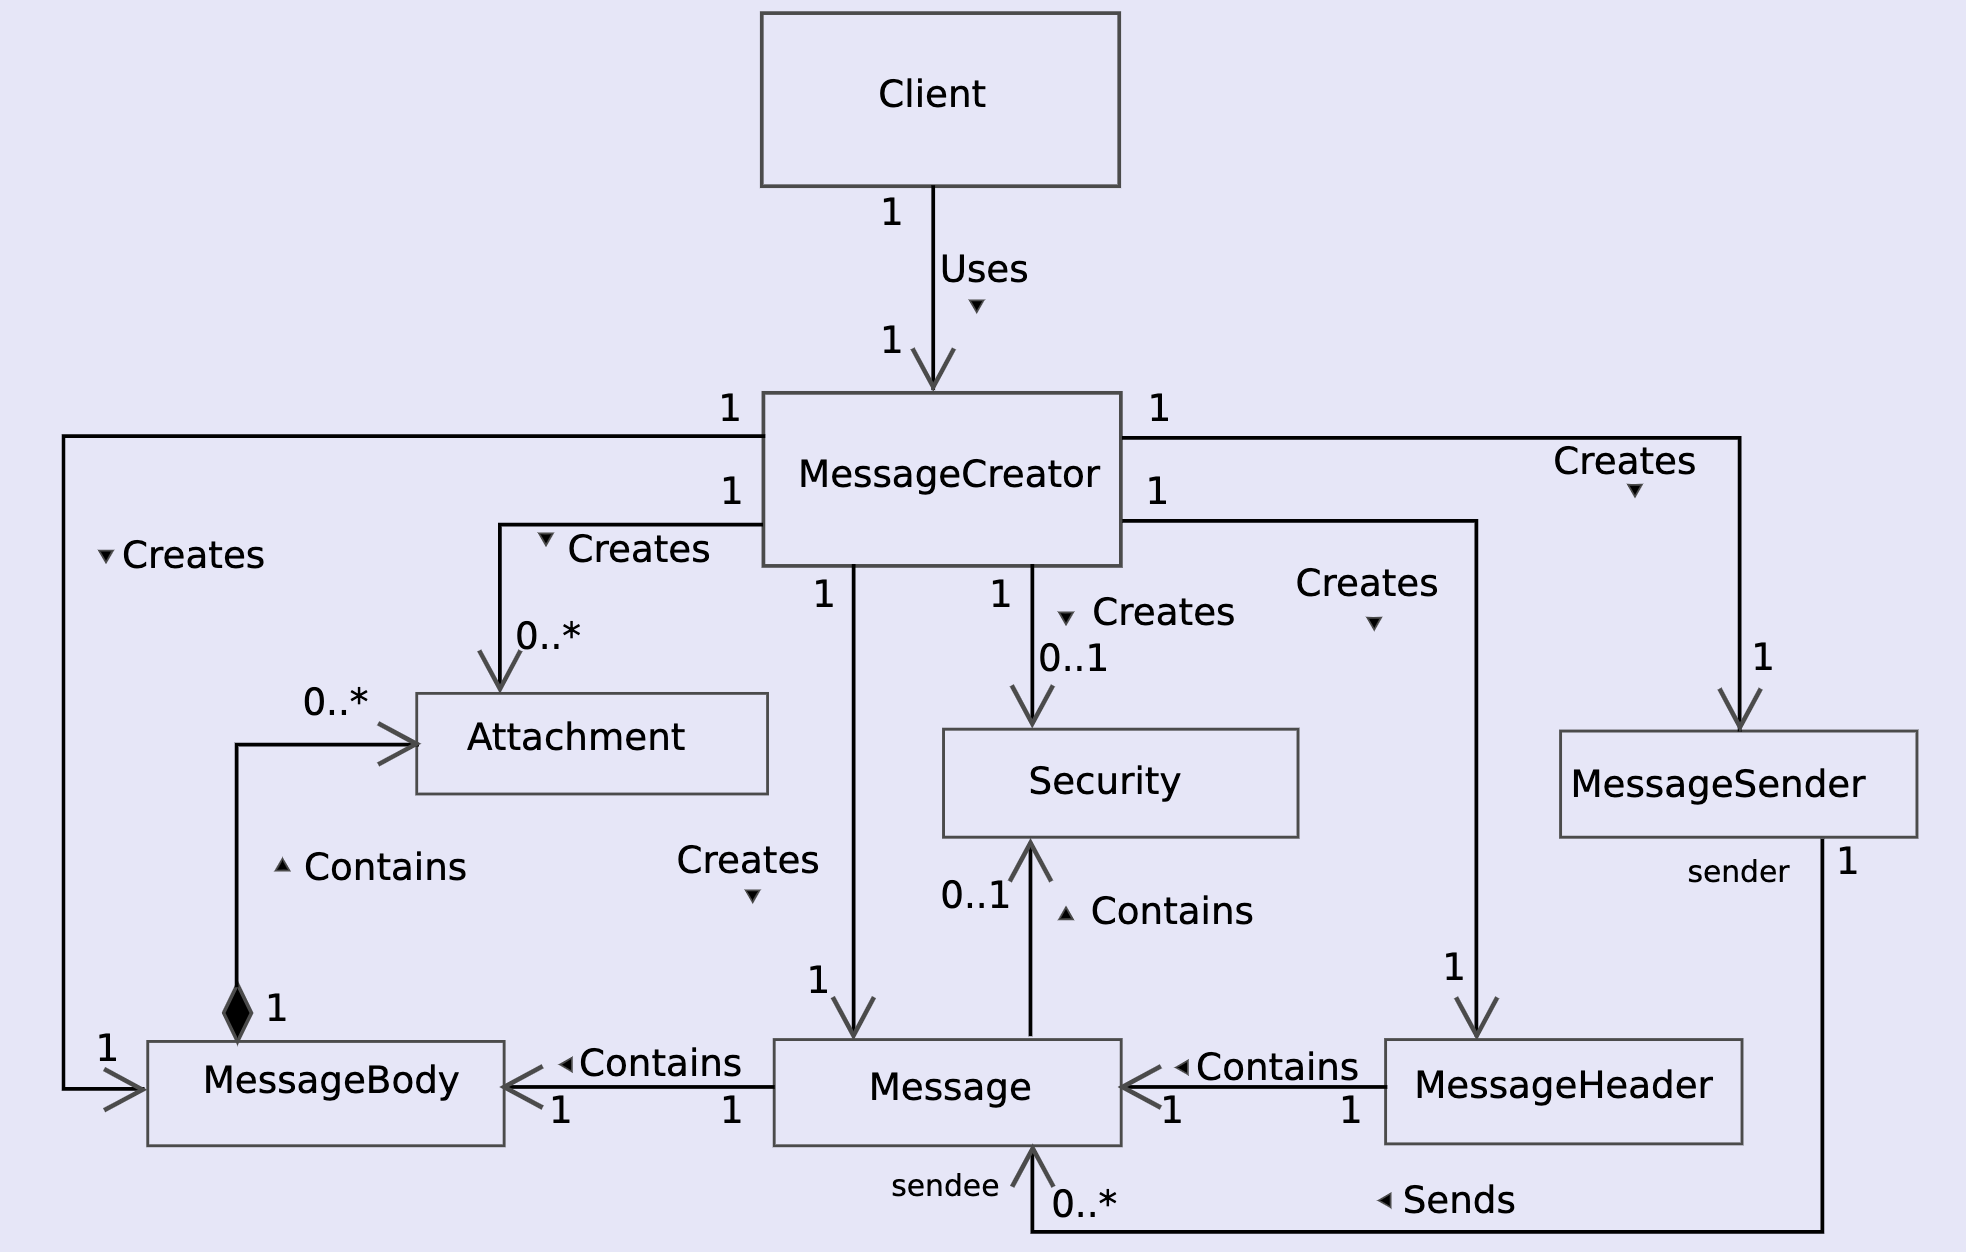
\includegraphics[width=1\linewidth]{assets/pattern/facade/facade-soluzione.png}
    \caption{Soluzione con pattern Façade}
\end{figure}

Il pattern permette quindi di nascondere ai client i componenti del sottosistema, riducendo il numero degli oggetti con cui i client interagiscono. Promuove il \textbf{basso accoppiamento} tra sottosistema e client, e \textbf{alta coesione} interna. Riduce le dipendenze di compilazione e non impedisce l'utilizzo delle classi del sottosistema qualora fosse necessario.

È utile sapere che un'interfaccia che implementa il pattern Façade può facilmente finire per essere accoppiata a tuttle le classi di un applicativo.

\newpage